\documentclass[11pt]{article}

\usepackage[a4paper,margin=22mm]{geometry}
\usepackage[T1]{fontenc}
\usepackage[utf8]{inputenc}
\usepackage{lmodern}
\usepackage{microtype}
\usepackage{amsmath,amssymb,mathtools}
\usepackage{booktabs}
\usepackage{graphicx}
\usepackage{enumitem}
\usepackage{algorithm2e}
\usepackage{tikz}
\usetikzlibrary{arrows.meta,positioning,shapes.geometric,fit,calc,backgrounds}
\usepackage[hidelinks]{hyperref}
\usepackage[nameinlink]{cleveref}
\usepackage{xcolor}

\definecolor{phaseblue}{RGB}{227,239,252}
\definecolor{phasegreen}{RGB}{228,244,233}
\definecolor{phaseorange}{RGB}{252,238,219}
\definecolor{phasegray}{RGB}{240,240,240}
\definecolor{phasepurple}{RGB}{239,231,250}
\definecolor{rejectred}{RGB}{252,229,229}

\SetKwComment{Comment}{$\triangleright$\ }{}
\SetAlgoLined
\DontPrintSemicolon
\newcommand{\D}{\mathbb D}
\newcommand{\R}{\mathbb R}
\newcommand{\E}{\mathrm E}
\newcommand{\area}{\operatorname{area}}
\newcommand{\interior}{\operatorname{int}}
\newcommand{\dist}{\operatorname{dist}}
\newcommand{\Id}{\mathrm{Id}}
\newcommand{\Bz}{\mathcal B}
\newcommand{\KB}{\mathcal K}

\title{A Concrete Search Algorithm for Strong Stein Monohedral Tilings of the Disk}
\author{Algorithmic design note}
\date{August 2026}

\begin{document}
\maketitle

\begin{abstract}
This document specifies an executable search architecture for the strong form of Stein's disk tiling problem: partition the unit disk into finitely many congruent topological disks, with the center lying in the interior of one tile. The design is intentionally narrower than an unrestricted search over arbitrary Jordan curves. It introduces a finite hierarchy of boundary models, a finite search routine \textsc{Stein-Search}$(B)$ for each complexity budget $B$, and an outer dovetailing scheduler that increases both tile count and representation complexity. The core pipeline is: enumerate a combinatorial contact schema; contract the Euclidean placement variables; run two independent relaxations in parallel; synthesize a boundary in a schema-aware parameterization; and certify the resulting packing with interval methods. Certified failures feed back as logically valid no-good constraints, while merely numerical failures affect ranking but never prune the exact search space.
\end{abstract}

\section{Problem and exact target}

Let
\[
\D=\{x\in\R^2:\|x\|\le 1\}.
\]
We seek a topological disk $T\subset\R^2$ and Euclidean isometries
\[
 g_i(x)=Q_i x+t_i,\qquad Q_i\in O(2),\qquad i=1,\ldots,n,
\]
such that
\begin{align}
\D &= \bigcup_{i=1}^n g_i(T), \\
\interior(g_iT)\cap\interior(g_jT)&=\varnothing\qquad(i\ne j), \\
0&\in\interior(g_1T).
\end{align}
We fix the gauge
\[
g_1=\Id,
\]
so the prototype itself is the center-containing tile.

The algorithm searches for a \emph{packing of full area}, not for coverage directly. If every $g_i(T)$ is contained in $\D$, their interiors are pairwise disjoint, $T$ has piecewise-regular Jordan boundary, and
\[
\area(T)=\frac{\pi}{n},
\]
then the finite union has the same area as $\D$. Because the union is closed, a nonempty complement in $\D$ would contain a relatively open set of positive area. Hence the packing is a tiling.

\subsection{The placement variables used by the search}

Define the preimage of the disk center under copy $i$ by
\[
c_i:=g_i^{-1}(0)=-Q_i^Tt_i.
\]
Equivalently,
\[
g_i(x)=Q_i(x-c_i).
\]
Then $c_1=0$. Containment of every copy in the unit disk is equivalent to
\[
T\subseteq B(c_i,1)\qquad\text{for every }i,
\]
and therefore
\begin{equation}
\boxed{T\subseteq K(C):=\bigcap_{i=1}^n B(c_i,1).}
\label{eq:lens}
\end{equation}
If a boundary arc of $T$ is exposed on the outer circle by copy $i$, then that prototype arc must lie exactly on
\[
\partial B(c_i,1).
\]
This is the main geometric reduction used throughout the algorithm.

\begin{figure}[ht]
\centering
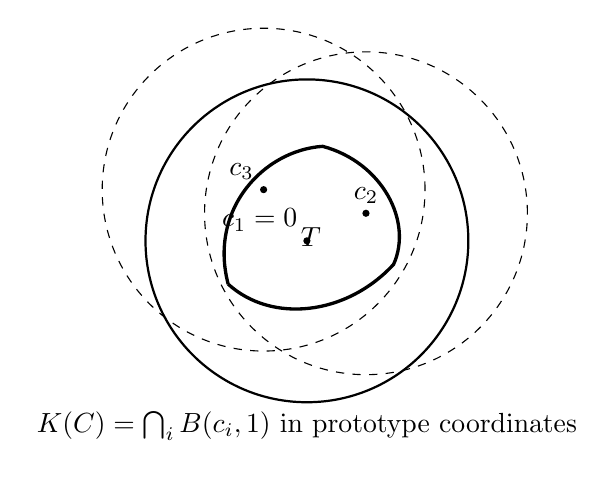
\begin{tikzpicture}[scale=1.0]
  \draw[thick] (0,0) circle (2.05);
  \node at (0,-2.35) {$K(C)=\bigcap_i B(c_i,1)$ in prototype coordinates};
  \fill (0,0) circle (1.3pt) node[above left] {$c_1=0$};
  \fill (0.75,0.35) circle (1.3pt) node[above] {$c_2$};
  \fill (-0.55,0.65) circle (1.3pt) node[above left] {$c_3$};
  \draw[dashed] (0.75,0.35) circle (2.05);
  \draw[dashed] (-0.55,0.65) circle (2.05);
  \draw[very thick] (-1.00,-0.55) .. controls (-0.45,-1.05) and (0.50,-0.95) .. (1.10,-0.30)
       .. controls (1.35,0.25) and (0.95,1.00) .. (0.20,1.20)
       .. controls (-0.55,1.15) and (-1.25,0.40) .. (-1.00,-0.55);
  \node at (0.05,0.05) {$T$};
\end{tikzpicture}
\caption{The prototype is searched inside an intersection of unit disks centered at the preimages $c_i$ of the global center. Dashed circles indicate two of the containment constraints.}
\label{fig:lens}
\end{figure}

\section{Finite representation hierarchy}

An unrestricted search over arbitrary Jordan curves is not an algorithm. We therefore define a hierarchy indexed by a complexity budget $B$.

For fixed $B$, the prototype boundary is a cyclic sequence of at most $m_{\max}(B)$ \emph{atoms}. Each atom is one of two types.

\begin{enumerate}[label=\textbf{A\arabic*.},leftmargin=16mm]
\item \textbf{Exposed circular atom.} It is labeled by a copy index $i$ and is constrained to lie on $\partial B(c_i,1)$. It is represented by its ordered endpoints on that circle.
\item \textbf{Interface atom.} It belongs to a paired interface class. One occurrence is a master polynomial Bezier arc of degree at most $d_{\max}(B)$; the mate is generated exactly by a relative Euclidean isometry $h_{ij}=g_i^{-1}g_j$ and an optional parameter reversal. Thus congruence of the two sides of an interface is built into the parameterization rather than penalized numerically.
\end{enumerate}

A \emph{contact schema} records:
\begin{itemize}[leftmargin=7mm]
\item a finite planar cell-complex type with $n$ tile faces and one exterior face;
\item the cyclic order of boundary atoms on the prototype;
\item which prototype atoms are exposed by which copies;
\item which interface atoms are paired, and the corresponding copy-pair labels;
\item the incidence pattern of interface endpoints and multiple junctions;
\item a reflection bit $r_i\in\{0,1\}$ for every copy, with
\[
Q_i=R_i F^{r_i},\qquad F=\begin{pmatrix}-1&0\\0&1\end{pmatrix},
\]
where $R_i$ is an unknown rotation represented algebraically by $(a_i,b_i)$ satisfying $a_i^2+b_i^2=1$.
\end{itemize}

Every round has finite bounds on $n$, the number of atoms, Bezier degree, junction degree, branch-and-bound depth, grid size, moment order, number of optimization evaluations, and certification subdivisions. Consequently every call \textsc{Stein-Search}$(B)$ terminates.

\section{Global architecture}

The search is organized around a single immutable candidate identity
\[
\chi=(n,S,P,W,Z),
\]
where $S$ is a contact schema, $P$ is a box of placement parameters, $W$ is an optional coarse indicator witness, and $Z$ is an explicit boundary parameter vector. Not every stage fills every field.

\begin{figure}[p]
\centering
\resizebox{0.96\textwidth}{!}{%
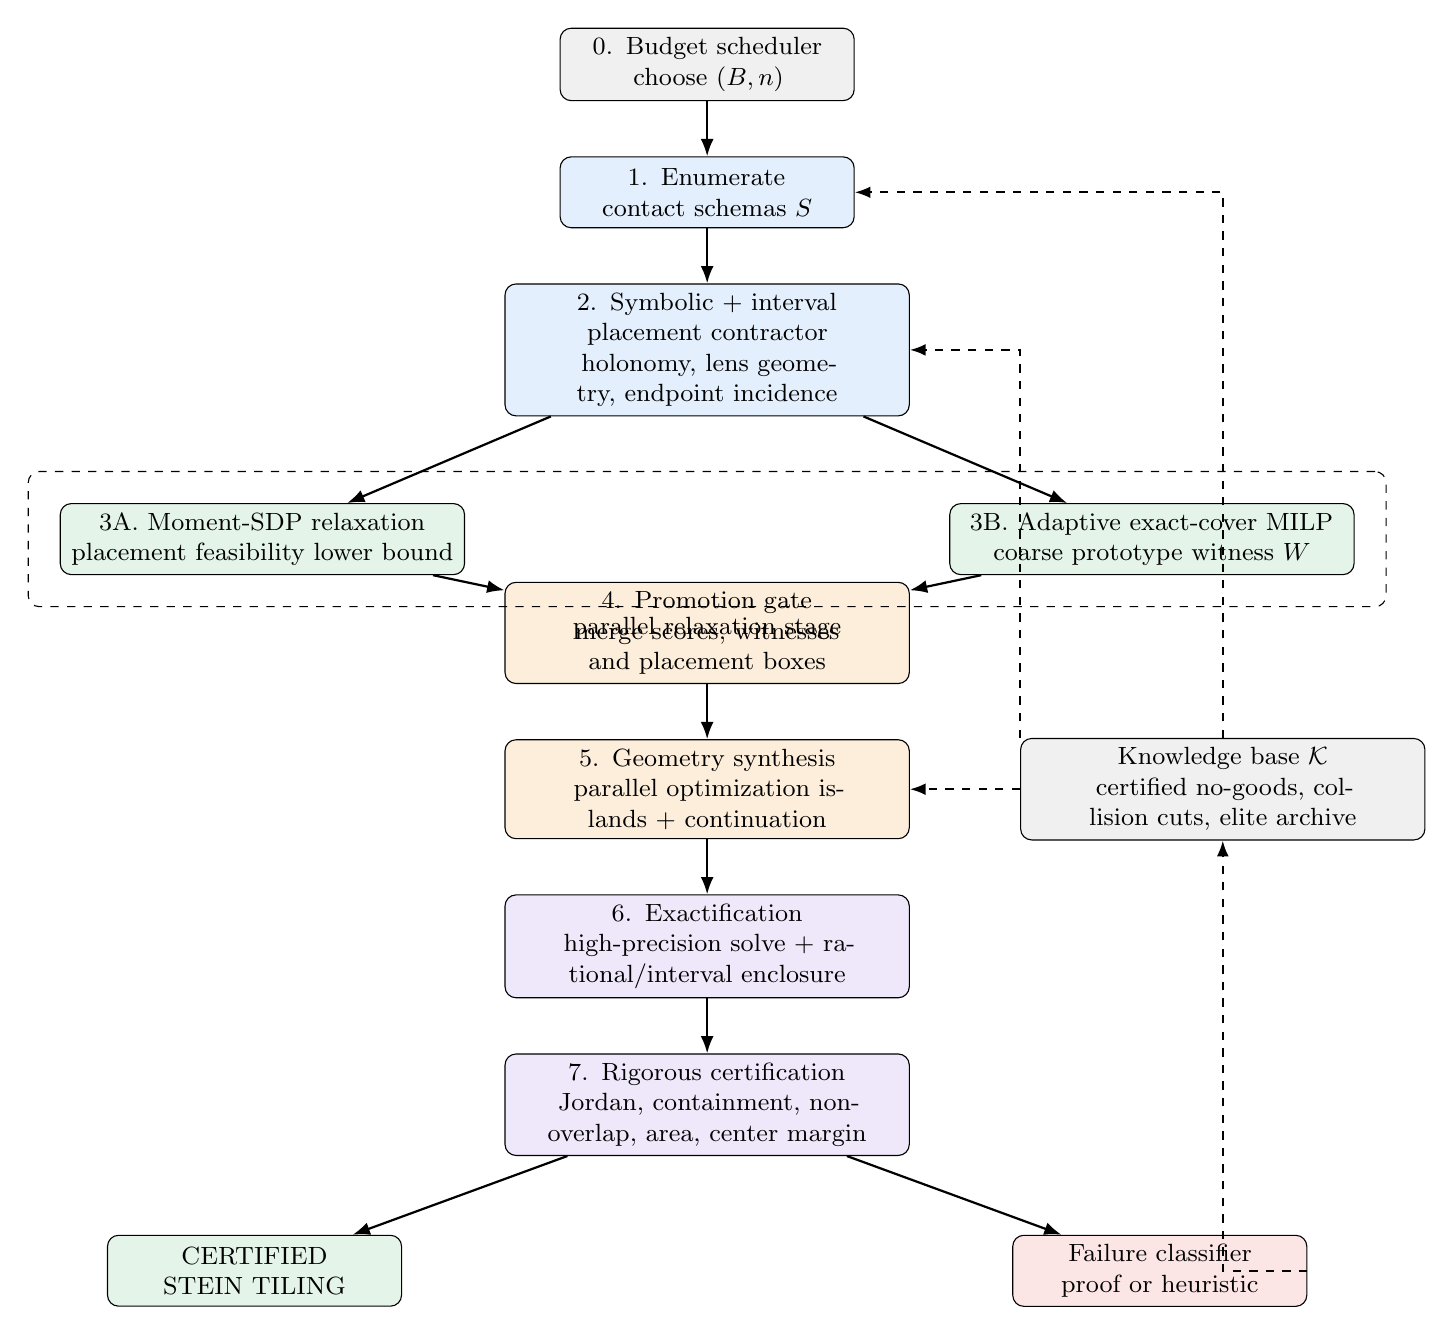
\begin{tikzpicture}[
  node distance=7mm and 10mm,
  box/.style={draw,rounded corners,align=center,minimum height=9mm,text width=35mm,font=\small},
  wide/.style={draw,rounded corners,align=center,minimum height=9mm,text width=49mm,font=\small},
  arr/.style={-{Latex[length=2.2mm]},thick},
  fb/.style={-{Latex[length=2mm]},thick,dashed}
]
  \node[box,fill=phasegray] (sched) {0. Budget scheduler\\choose $(B,n)$};
  \node[box,fill=phaseblue,below=of sched] (enum) {1. Enumerate\\contact schemas $S$};
  \node[wide,fill=phaseblue,below=of enum] (contract) {2. Symbolic + interval placement contractor\\holonomy, lens geometry, endpoint incidence};

  \node[wide,fill=phasegreen,below left=11mm and 5mm of contract] (mom) {3A. Moment-SDP relaxation\\placement feasibility lower bound};
  \node[wide,fill=phasegreen,below right=11mm and 5mm of contract] (grid) {3B. Adaptive exact-cover MILP\\coarse prototype witness $W$};

  \node[wide,fill=phaseorange,below=21mm of contract] (fusion) {4. Promotion gate\\merge scores, witnesses and placement boxes};
  \node[wide,fill=phaseorange,below=of fusion] (synth) {5. Geometry synthesis\\parallel optimization islands + continuation};
  \node[wide,fill=phasepurple,below=of synth] (exact) {6. Exactification\\high-precision solve + rational/interval enclosure};
  \node[wide,fill=phasepurple,below=of exact] (cert) {7. Rigorous certification\\Jordan, containment, non-overlap, area, center margin};

  \node[box,fill=phasegreen,below left=10mm and 13mm of cert] (success) {CERTIFIED\\STEIN TILING};
  \node[box,fill=rejectred,below right=10mm and 13mm of cert] (fail) {Failure classifier\\proof or heuristic};
  \node[wide,fill=phasegray,right=14mm of synth] (kb) {Knowledge base $\KB$\\certified no-goods, collision cuts, elite archive};

  \draw[arr] (sched)--(enum);
  \draw[arr] (enum)--(contract);
  \draw[arr] (contract)--(mom);
  \draw[arr] (contract)--(grid);
  \draw[arr] (mom)--(fusion);
  \draw[arr] (grid)--(fusion);
  \draw[arr] (fusion)--(synth);
  \draw[arr] (synth)--(exact);
  \draw[arr] (exact)--(cert);
  \draw[arr] (cert)--(success);
  \draw[arr] (cert)--(fail);

  \draw[fb] (fail.east) -| (kb.south);
  \draw[fb] (kb.north) |- (enum.east);
  \draw[fb] (kb.west) -- (synth.east);
  \draw[fb] (kb.north west) |- (contract.east);

  \node[draw,dashed,rounded corners,fit=(mom)(grid),inner sep=4mm,label={[font=\small]below:parallel relaxation stage}] {};
\end{tikzpicture}%
}
\caption{The complete search pipeline. Only logically certified information is allowed to prune future exact search. Numerical information may seed or rank candidates but cannot delete a branch.}
\label{fig:pipeline}
\end{figure}

\section{Stage 1: finite combinatorial enumeration}

For each pair $(B,n)$, enumerate all schemas satisfying the hard combinatorial rules within the current bounds. The enumeration is canonicalized under relabeling so isomorphic schemas are produced once.

Immediate rejection rules include:
\begin{itemize}[leftmargin=7mm]
\item the prototype boundary is not one cyclic component;
\item the induced tile face is not a topological disk;
\item the planar incidence data violate Euler relations;
\item an interface atom is not paired exactly once;
\item local junction incidences cannot be paired consistently across congruent copies;
\item a schema contains a certified no-good already stored in $\KB$.
\end{itemize}

This stage deliberately does \emph{not} require normality of the tiling. Non-normal junction patterns are permitted whenever they fit the finite incidence budget.

\section{Stage 2: symbolic and interval placement contraction}

For a surviving schema, define placement variables
\[
P=\{c_i,a_i,b_i,r_i\}_{i=1}^n,
\qquad c_1=0,\quad (a_1,b_1)=(1,0),\quad r_1=0.
\]
The reflection bits are discrete and already fixed in the schema; the remaining variables are continuous.

The contractor applies four classes of constraints.

\paragraph{C1. Orthogonality.}
\[
a_i^2+b_i^2=1.
\]

\paragraph{C2. Lens feasibility.}
Every prototype point must lie in $K(C)$ from \cref{eq:lens}. Before the prototype is known, use necessary conditions including a lower bound on the area of $K(C)$:
\[
\area(K(C))\ge \frac{\pi}{n},
\]
and a positive center-margin variable $\rho$ satisfying
\[
B(0,\rho)\subseteq K(C).
\]
The search maximizes $\rho$ later; here we only require $\rho\ge\rho_{\min}(B)>0$ for promoted boxes, while boxes with smaller unresolved margins can be deferred to a later budget.

\paragraph{C3. Euclidean gain and holonomy constraints.}
For every interface between copies $i$ and $j$, form
\[
h_{ij}=g_i^{-1}g_j.
\]
Endpoint identifications and cycles in the contact complex yield fixed-point or coincidence equations. Around every combinatorial junction cycle, compose the corresponding gains and require the resulting isometry to be compatible with the designated junction point. Contradictory translation/rotation/reflection types reject the branch immediately.

\paragraph{C4. Exposed-arc incidence.}
If prototype atom $A$ is exposed by copy $i$, both endpoints of $A$ are constrained to $\partial B(c_i,1)$. If the same prototype endpoint belongs to two exposed atoms labeled $i$ and $j$, it lies in
\[
\partial B(c_i,1)\cap\partial B(c_j,1),
\]
which gives an algebraic distance constraint on $c_i-c_j$.

The continuous search is interval branch-and-bound to a fixed depth $L_{\max}(B)$. A node is rejected only when interval contraction proves emptiness. Surviving placement boxes are passed to Stage 3.

\section{Stage 3: two relaxations in parallel}

The two branches answer different questions and are intentionally independent.

\subsection{Branch 3A: truncated moment-SDP feasibility}

Introduce unknown prototype moments
\[
\mu_{pq}=\int_T x_1^p x_2^q\,dx,
\qquad p+q\le M(B).
\]
For each disk moment $m_{pq}(\D)$, the exact tiling identity implies
\[
m_{pq}(\D)=\sum_{i=1}^n\int_T \bigl(g_i(x)_1\bigr)^p\bigl(g_i(x)_2\bigr)^q\,dx.
\]
For fixed placement parameters this is linear in the $\mu_{pq}$. Over a placement box, interval coefficients are used. Add:
\begin{itemize}[leftmargin=7mm]
\item $\mu_{00}=\pi/n$;
\item positive-semidefinite moment matrix constraints;
\item localizing constraints derived from support in $K(C)$;
\item optional higher-order symmetry cancellation equations inherited from the radial moments of the disk.
\end{itemize}

If the semidefinite relaxation is rigorously infeasible, the placement box is rejected. Otherwise it receives a feasibility lower bound and proceeds.

\subsection{Branch 3B: adaptive exact-cover MILP}

Choose a finite adaptive partition $\mathcal G_B$ of a bounding region containing every possible prototype in the current placement box. Associate a binary variable $u_q$ to each prototype cell $q$.

At sample points $x_k\in\D$, approximate
\[
\sum_{i=1}^n \mathbf 1_T(g_i^{-1}x_k)=1
\]
by the discrete constraints
\[
\sum_{i=1}^n u_{q(i,k)}=1,
\]
whenever every transformed sample $g_i^{-1}x_k$ falls unambiguously in a prototype cell. Ambiguous samples caused by interval placement boxes are postponed or refined.

Additional discrete constraints enforce:
\begin{itemize}[leftmargin=7mm]
\item a connected selected-cell set;
\item a connected complement inside a local enclosing box, suppressing holes;
\item selected cells around the origin, providing an interior-center seed;
\item approximate area $\sum_q u_q\area(q)\approx\pi/n$;
\item forbidden cells outside the interval enclosure of $K(C)$.
\end{itemize}

A feasible MILP returns a coarse witness $W$, which is not a proof and is never used alone to prune. It is used to initialize the explicit boundary in Stage 5.

\section{Stage 4: promotion gate}

A placement box is promoted to geometry synthesis if:
\begin{enumerate}[leftmargin=9mm]
\item neither the symbolic contractor nor the moment-SDP branch has proved it impossible; and
\item either the exact-cover branch has produced a witness, or the moment relaxation is unusually strong and the box is among the top $R(B)$ placements by score.
\end{enumerate}

The gate forms a record
\[
\chi=(n,S,P,W,\varnothing)
\]
and pushes it into a priority queue. Priority is based on:
\begin{itemize}[leftmargin=7mm]
\item certified lower bound on possible center margin;
\item exact-cover residual and boundary complexity of $W$;
\item moment-relaxation slack;
\item novelty relative to the elite archive.
\end{itemize}
No priority score is logically authoritative.

\section{Stage 5: explicit geometry synthesis}

The schema is now converted into a low-dimensional boundary model.

\subsection{Schema-aware boundary parameterization}

For every exposed atom labeled $i$, the curve is an exact unit-circle arc centered at $c_i$. Only its endpoints and orientation are variables.

For every interface pair, introduce exactly one master Bezier curve
\[
\gamma(s)=\sum_{k=0}^{d} P_k B_{k,d}(s),\qquad 0\le s\le1,
\]
with $d\le d_{\max}(B)$. Its mate is not independently optimized: it is generated as
\[
\widetilde\gamma(s)=h_{ij}\bigl(\gamma(s)\bigr)
\quad\text{or}\quad
\widetilde\gamma(s)=h_{ij}\bigl(\gamma(1-s)\bigr),
\]
as specified by the schema. Thus interface congruence is exact at every numerical iterate.

\subsection{Optimization objective}

Let $Z$ collect placement variables, arc endpoints, and master-curve control points. Define
\begin{equation}
\mathcal L(Z)=
\lambda_{\mathrm{out}}E_{\mathrm{out}}
+\lambda_{\mathrm{over}}E_{\mathrm{over}}
+\lambda_{\mathrm{area}}E_{\mathrm{area}}
+\lambda_{\mathrm{inc}}E_{\mathrm{inc}}
+\lambda_{\mathrm{reg}}E_{\mathrm{reg}}
-\lambda_{\rho}\rho(Z).
\label{eq:loss}
\end{equation}
Here:
\begin{align*}
E_{\mathrm{out}}&:\ \text{penalty for }T\not\subseteq K(C),\\
E_{\mathrm{over}}&:\ \text{pairwise interior-overlap integral of the copies},\\
E_{\mathrm{area}}&=\left(\area(T)-\frac{\pi}{n}\right)^2,\\
E_{\mathrm{inc}}&:\ \text{junction and endpoint incidence residual},\\
E_{\mathrm{reg}}&:\ \text{curvature and control-polygon regularization},\\
\rho(Z)&=\dist(0,\partial T).
\end{align*}
The optimizer is not asked to fit coverage: full coverage will follow from the certified packing and exact area condition.

\subsection{Parallel island optimizer}

For each promoted record, create $I(B)$ optimization islands. Initialization is split between:
\begin{itemize}[leftmargin=7mm]
\item boundary fits extracted from the coarse witness $W$;
\item randomized perturbations within the placement box $P$;
\item elite candidates from nearby schemas or previous budgets.
\end{itemize}
Each island alternates:
\begin{enumerate}[leftmargin=9mm]
\item global derivative-free moves on the low-dimensional placement variables;
\item local gradient-based minimization of all continuous boundary variables;
\item geometric continuation from coarse collision quadrature to finer quadrature.
\end{enumerate}
Every $G(B)$ generations, islands exchange only their best few candidates through the elite archive. The run has a fixed evaluation limit, so it terminates.

A candidate is sent to exactification if all numerical residuals fall below budget-dependent thresholds and $\rho$ is positive by a comfortable numerical margin.

\begin{figure}[ht]
\centering
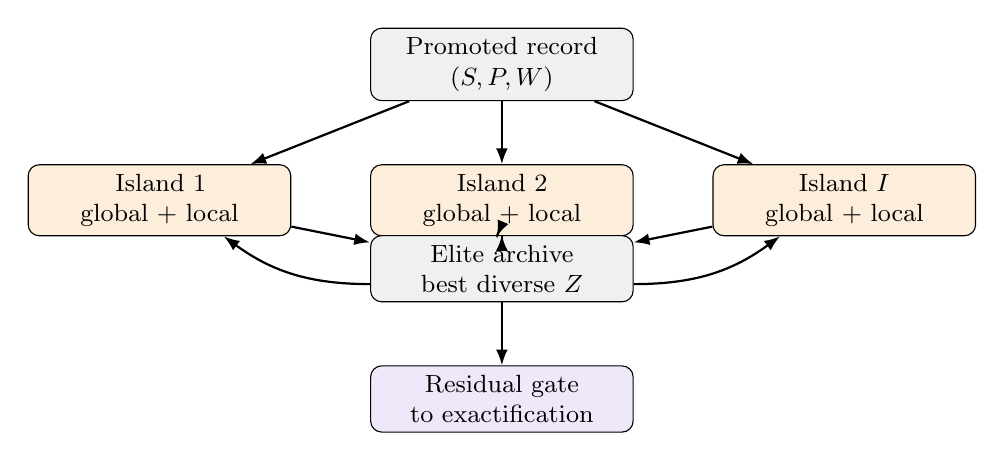
\begin{tikzpicture}[
  node distance=8mm and 10mm,
  box/.style={draw,rounded corners,align=center,minimum height=8mm,text width=31mm,font=\small},
  arr/.style={-{Latex[length=2mm]},thick}
]
  \node[box,fill=phasegray] (seed) {Promoted record\\$(S,P,W)$};
  \node[box,fill=phaseorange,below left=of seed] (i1) {Island 1\\global + local};
  \node[box,fill=phaseorange,below=of seed] (i2) {Island 2\\global + local};
  \node[box,fill=phaseorange,below right=of seed] (ik) {Island $I$\\global + local};
  \node[box,fill=phasegray,below=17mm of seed] (archive) {Elite archive\\best diverse $Z$};
  \node[box,fill=phasepurple,below=of archive] (promote) {Residual gate\\to exactification};
  \draw[arr] (seed)--(i1); \draw[arr] (seed)--(i2); \draw[arr] (seed)--(ik);
  \draw[arr] (i1)--(archive); \draw[arr] (i2)--(archive); \draw[arr] (ik)--(archive);
  \draw[arr,bend left=18] (archive) to (i1);
  \draw[arr] (archive) to[bend left=8] (i2);
  \draw[arr,bend right=18] (archive) to (ik);
  \draw[arr] (archive)--(promote);
\end{tikzpicture}
\caption{Stage 5 is parallel but bounded. It is a candidate generator, not a proof engine.}
\label{fig:islands}
\end{figure}

\section{Stage 6: exactification}

Numerical parameters are converted to a certifiable local problem.

\begin{enumerate}[leftmargin=9mm]
\item Replace rotation angles by algebraic variables $(a_i,b_i)$ with $a_i^2+b_i^2=1$.
\item Express all endpoint incidences, circle incidences, interface pairings, and the area condition as a finite system
\[
F(z)=0.
\]
\item Increase arithmetic precision and apply Newton or constrained least squares to obtain a high-precision approximate root $z_0$.
\item Form a rational interval box $X$ around $z_0$.
\item Use interval Newton or a Krawczyk operator. If it proves that $F$ has a unique root in $X$, retain $X$ as the exact parameter enclosure. Otherwise subdivide up to the current exactification budget. Failure here does not prove that the schema is impossible unless interval methods exclude the entire parent parameter box.
\end{enumerate}

The area constraint is evaluated by Green's theorem. Circular atoms have analytic line integrals; polynomial Bezier atoms have polynomial line integrals. Hence $\area(T)$ is a finite explicit expression in the certified parameters and $\pi$.

\section{Stage 7: rigorous geometric certificate}

A successful exactification box $X$ is accepted only after every property below is proved with directed interval arithmetic.

\begin{enumerate}[label=\textbf{V\arabic*.},leftmargin=16mm]
\item \textbf{Jordan property.} Adjacent boundary atoms meet only at their prescribed common endpoint. Nonadjacent atoms are disjoint. Bezier convex-hull subdivision and exact circular-arc bounding boxes are recursively refined until separation is proved.
\item \textbf{Positive center margin.} Prove
\[
\dist(0,\partial T)>0
\]
and orient the Jordan curve so the origin is in its interior.
\item \textbf{Containment.} Prove
\[
T\subseteq B(c_i,1)
\qquad \forall i.
\]
Since $g_i(x)=Q_i(x-c_i)$, this proves $g_i(T)\subseteq\D$.
\item \textbf{Pairwise packing.} For every $i<j$, prove
\[
\interior(T)\cap\interior(h_{ij}T)=\varnothing.
\]
Prescribed interface atoms are allowed to coincide; all other boundary and interior regions must be separated. A certified planar arrangement test determines the relative inside/outside relation.
\item \textbf{Exact area.} Prove, through the certified root of $F$, that
\[
\area(T)=\frac{\pi}{n}.
\]
\end{enumerate}

If V1--V5 hold, output the boundary atoms, the interval-enclosed placements, and the verification transcript. This constitutes a computer-assisted proof of a strong monohedral tiling.

\section{Feedback and learning}

The failure classifier distinguishes \emph{proof-producing} information from \emph{heuristic} information.

\begin{table}[ht]
\centering
\small
\begin{tabular}{p{36mm}p{47mm}p{54mm}}
\toprule
Failure source & Returned object & Permitted effect \\
\midrule
Symbolic contradiction & Minimal inconsistent schema constraints & Permanent no-good on schemas \\
Interval placement exclusion & Certified empty placement box & Permanent geometric cut \\
Moment-SDP infeasibility & Dual infeasibility certificate, when validated & Permanent placement cut \\
Certified collision & Interval witness identifying atom/copy pair & Add collision cut; re-optimize siblings \\
MILP infeasibility & Discrete-grid fact only & Ranking/defer only; never exact pruning \\
Optimizer stagnation & Numerical statistics & Ranking/reseeding only \\
Exactification failure without exclusion & No proof & Increase precision/budget or defer \\
\bottomrule
\end{tabular}
\caption{Only certified statements are allowed to shrink the exact search space. This prevents an optimization artifact from silently turning into a mathematical assumption.}
\label{tab:feedback}
\end{table}

The knowledge base $\KB$ therefore has three typed stores:
\[
\KB=(\KB_{\mathrm{proof}},\KB_{\mathrm{cuts}},\KB_{\mathrm{elite}}).
\]
The first two may prune only within the domains for which their certificates are valid. The elite archive is purely heuristic.

\section{Master algorithm}

\begin{algorithm}[p]
\caption{\textsc{Stein-Search}$(B)$: one finite search round}
\label{alg:round}
\KwIn{Complexity budget $B$; persistent knowledge base $\KB$}
\KwOut{A certified tiling, or \textsc{NoCandidateAtBudget}}

Compute finite bounds $N_{\max},m_{\max},d_{\max},L_{\max},M,R,I,G,E_{\max}$ from $B$\;
Initialize priority queue $Q\leftarrow\varnothing$\;

\For{$n\leftarrow4$ \KwTo $N_{\max}$}{
  \ForEach{canonical schema $S\in\textsc{EnumerateSchemas}(n,B,\KB_{\mathrm{proof}})$}{
    $\mathcal P\leftarrow\textsc{ContractPlacements}(S,B,\KB_{\mathrm{cuts}})$\;
    \ForEach{surviving placement box $P\in\mathcal P$}{
      Run in parallel:\;
      \Indp
      $A\leftarrow\textsc{MomentRelaxation}(S,P,B)$\;
      $W\leftarrow\textsc{GridExactCover}(S,P,B)$\;
      \Indm
      \If{$A$ is certified infeasible}{
         Store validated cut in $\KB_{\mathrm{cuts}}$; \textbf{continue}\;
      }
      \If{\textsc{PromotionRule}$(A,W,P,B)$}{
         push $(n,S,P,W)$ into $Q$ with heuristic priority\;
      }
    }
  }
}

\While{$Q\ne\varnothing$ and synthesis evaluations $<E_{\max}$}{
  $(n,S,P,W)\leftarrow\textsc{PopBest}(Q)$\;
  $\mathcal Z\leftarrow\textsc{SynthesizeGeometry}(n,S,P,W,B,\KB_{\mathrm{elite}})$\;
  \ForEach{$Z\in\mathcal Z$ passing the numerical residual gate}{
    $X\leftarrow\textsc{Exactify}(n,S,Z,B)$\;
    \If{$X$ is a certified root enclosure}{
       $C\leftarrow\textsc{CertifyTiling}(n,S,X,B)$\;
       \If{$C$ is valid}{
          \Return{$C$}\;
       }
       \Else{
          \textsc{ClassifyAndStore}$(C,\KB)$\;
       }
    }
  }
}
\Return{\textsc{NoCandidateAtBudget}}\;
\end{algorithm}

The global driver is a dovetailing loop rather than a depth-first commitment to one tile count.

\begin{algorithm}[ht]
\caption{Unbounded dovetailing driver}
\label{alg:driver}
Initialize persistent knowledge base $\KB$\;
\For{$B\leftarrow1,2,3,\ldots$}{
  $C\leftarrow\textsc{Stein-Search}(B,\KB)$\;
  \If{$C$ is a certified tiling}{\Return{$C$}}
}
\end{algorithm}

Because every round is finite, the driver cannot become permanently trapped trying to exhaust all boundaries for $n=4$ before ever considering $n=5,6,\ldots$. The mapping from $B$ to bounds should satisfy
\[
N_{\max}(B),\ m_{\max}(B),\ d_{\max}(B),\ L_{\max}(B),\ M(B)\longrightarrow\infty.
\]

\section{Communication sequence}

\begin{figure}[p]
\centering
\resizebox{0.97\textwidth}{!}{%
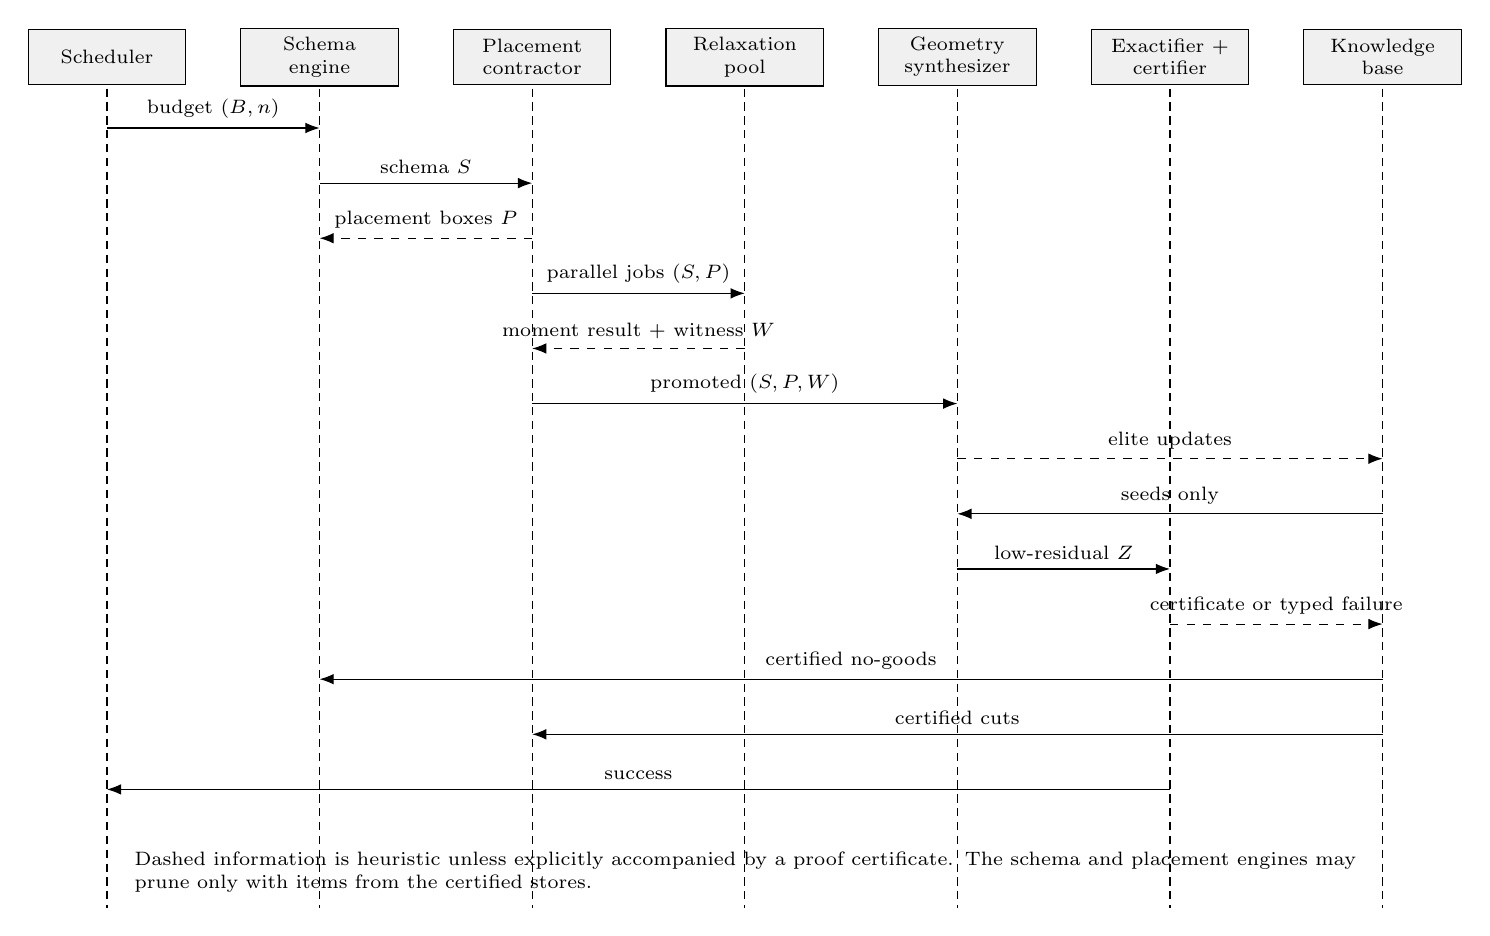
\begin{tikzpicture}[
  font=\scriptsize,
  lifeline/.style={draw,fill=phasegray,minimum width=20mm,minimum height=7mm,align=center},
  msg/.style={-{Latex[length=1.8mm]},thin},
  ret/.style={-{Latex[length=1.8mm]},thin,dashed}
]
  \node[lifeline] (sc) at (0,0) {Scheduler};
  \node[lifeline] (en) at (2.7,0) {Schema\\engine};
  \node[lifeline] (pc) at (5.4,0) {Placement\\contractor};
  \node[lifeline] (rl) at (8.1,0) {Relaxation\\pool};
  \node[lifeline] (sy) at (10.8,0) {Geometry\\synthesizer};
  \node[lifeline] (ce) at (13.5,0) {Exactifier +\\certifier};
  \node[lifeline] (kb) at (16.2,0) {Knowledge\\base};

  \foreach \x in {0,2.7,5.4,8.1,10.8,13.5,16.2} {\draw[densely dashed] (\x,-0.4)--(\x,-10.8);}

  \draw[msg] (0,-0.9)-- node[above]{budget $(B,n)$} (2.7,-0.9);
  \draw[msg] (2.7,-1.6)-- node[above]{schema $S$} (5.4,-1.6);
  \draw[ret] (5.4,-2.3)-- node[above]{placement boxes $P$} (2.7,-2.3);
  \draw[msg] (5.4,-3.0)-- node[above]{parallel jobs $(S,P)$} (8.1,-3.0);
  \draw[ret] (8.1,-3.7)-- node[above]{moment result + witness $W$} (5.4,-3.7);
  \draw[msg] (5.4,-4.4)-- node[above]{promoted $(S,P,W)$} (10.8,-4.4);
  \draw[ret] (10.8,-5.1)-- node[above]{elite updates} (16.2,-5.1);
  \draw[msg] (16.2,-5.8)-- node[above]{seeds only} (10.8,-5.8);
  \draw[msg] (10.8,-6.5)-- node[above]{low-residual $Z$} (13.5,-6.5);
  \draw[ret] (13.5,-7.2)-- node[above]{certificate or typed failure} (16.2,-7.2);
  \draw[msg] (16.2,-7.9)-- node[above]{certified no-goods} (2.7,-7.9);
  \draw[msg] (16.2,-8.6)-- node[above]{certified cuts} (5.4,-8.6);
  \draw[msg] (13.5,-9.3)-- node[above]{success} (0,-9.3);

  \node[align=left,text width=155mm] at (8.1,-10.35) {Dashed information is heuristic unless explicitly accompanied by a proof certificate. The schema and placement engines may prune only with items from the certified stores.};
\end{tikzpicture}%
}
\caption{Sequence-level communication. The key design rule is a strict type separation between certified pruning information and heuristic search information.}
\label{fig:sequence}
\end{figure}

\section{What makes this an algorithm rather than a collection of ideas}

The architecture makes the following choices explicit.

\begin{enumerate}[leftmargin=9mm]
\item \textbf{Search object.} The primary discrete object is a contact schema; the primary continuous object is a placement box in $(c_i,Q_i)$ variables; the boundary is synthesized only after both have survived finite relaxations.
\item \textbf{Order.} Topology comes first, then placement, then two cheap-to-medium relaxations, then expensive boundary synthesis, then exactification, then proof.
\item \textbf{Parallelism.} Only Stage 3 and the optimization islands in Stage 5 run in parallel. Their outputs are merged at explicit gates.
\item \textbf{Feedback.} Exact failure certificates flow backward to the earliest module that can use them. Heuristic failures never prune.
\item \textbf{Termination.} Every inner module has a finite budget in \textsc{Stein-Search}$(B)$. The outer driver increases $B$ forever unless a certificate is found.
\item \textbf{Acceptance.} There is exactly one success condition: an independently checkable geometric certificate satisfying V1--V5. A visually convincing or $10^{-12}$ numerical residual is not success.
\end{enumerate}

\section{Completeness and limitation}

The algorithm is complete only relative to its representation hierarchy. If a strong Stein tiling exists whose prototype boundary can be represented at some finite level by the allowed circular atoms and polynomial Bezier interface atoms, with finite contact complexity and with a nondegenerate positive center margin, then sufficiently large budgets contain that representation class. Assuming exhaustive schema enumeration, exhaustive interval placement branching, and complete interval certification inside each bounded class, the outer driver will eventually reach the corresponding class.

The algorithm does \emph{not} prove completeness for arbitrary pathological Jordan boundaries. Extending the result from the chosen hierarchy to every topological disk would require an independent regularity theorem showing that a solution may be assumed to have a boundary in a representable class. The search architecture deliberately keeps this mathematical issue separate from the computational one.

\section{Recommended implementation order}

A practical implementation should be built in the following order, because each step produces independently testable artifacts.

\begin{enumerate}[leftmargin=9mm]
\item Implement the placement model $g_i(x)=Q_i(x-c_i)$, exact relative isometries $h_{ij}$, and interval lens constraints.
\item Implement a restricted schema family with only ordinary pairwise interfaces and finite-valence junctions; validate canonical enumeration and gain-cycle propagation.
\item Implement the adaptive exact-cover oracle. This immediately provides visual coarse prototypes and is useful for debugging the placement model.
\item Implement schema-aware circular/Bezier boundary synthesis and the parallel island archive.
\item Implement the rigorous Jordan/containment/non-overlap checker. Before solving Stein, validate it on synthetic tilings with known geometry.
\item Add interval Newton/Krawczyk exactification and the exact area equation.
\item Add the moment-SDP branch as a placement accelerator.
\item Only then enlarge the schema generator to increasingly non-normal incidence types and higher degrees.
\end{enumerate}

The first scientifically meaningful milestone is therefore not ``solve Stein'', but:
\begin{quote}
For fixed $(n,m,d)$, exhaust a well-defined schema class; produce either a rigorously certified tiling or a machine-checkable list of excluded placement boxes and no-good schemas covering that finite class.
\end{quote}
That milestone turns the open-ended search into a sequence of finite, reproducible mathematical experiments.

\end{document}
